%% Settings for single-side (simplex) printing
% Margins: left 40mm, right 25mm, top and bottom 25mm
% (but beware, LaTeX adds 1in implicitly)
\documentclass[12pt,a4paper]{report}
\setlength\textwidth{160mm}

\usepackage[utf8]{inputenc}
\usepackage{graphicx}
\usepackage{fancyhdr}
\usepackage{lmodern}
\usepackage{lastpage}
\usepackage{subfig}
\usepackage{hyperref}

\graphicspath{{../graphs/}}

\pagestyle{fancy}
\fancyhf{}
\rhead{Petr Houška `houskape@gmail.com`}
\lhead{HW2: Fibonacci heap}
\rfoot{Page \thepage / \pageref{LastPage}}


\begin{document}
	
	\begin{figure}[h]	
		\centering	
		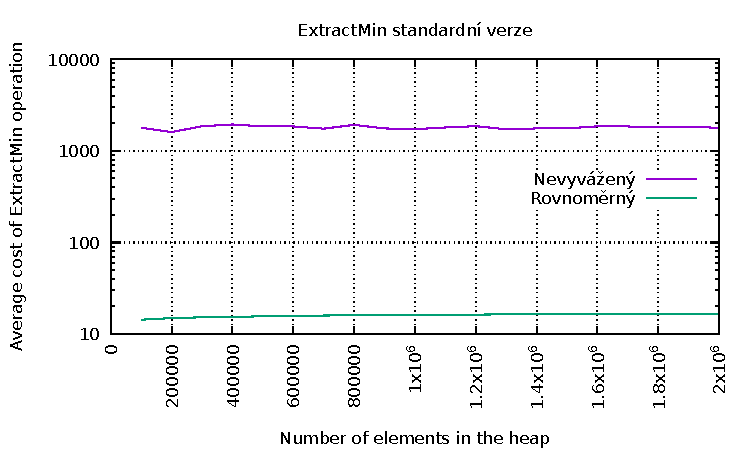
\includegraphics[scale=1.1]{graph_1}		
	\end{figure}

	\begin{figure}[h]	
    \centering
		\subfloat{{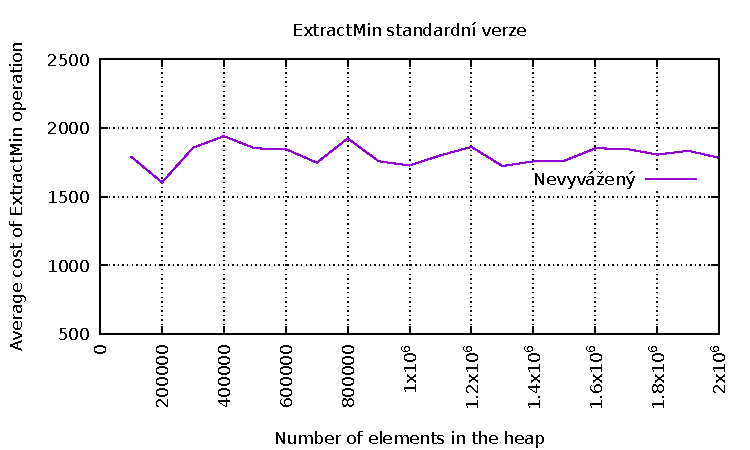
\includegraphics[scale=0.55]{graph_1_1}	 }}%
		\qquad
		\subfloat{{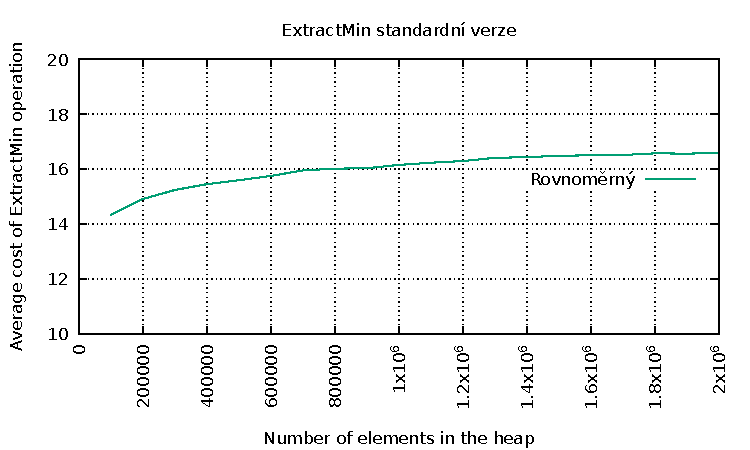
\includegraphics[scale=0.55]{graph_1_2}	}}%
    \end{figure}

První sada grafů ukazuje počet kroků ExtractMin v rámci dvou různých, náhodných posloupností operací, které se liší pouze podílem operace ExtractMin. Jsou na ní patrné dva zajímavé úkazy. 

Z grafu pro rovnoměrnou posloupnost je vidět, že počet kroků s rostoucí velikostí haldy pomalu roste. Z grafu se zdá, že by růst mohl být přibližně logaritmický. To by bylo konsistentní s faktem, že operace ExtractMin má mít amortizovanou logaritmickou časovou složitost a že námi počítané kroky jsou podmnožina operací, které musí ExtractMin provést (nezapočítáváme například stromy z haldového lesa, které v něm byly ještě před odebrání minima a které s žádným jiným v rámci konsolidace nespojujeme). Základ logaritmu je, zřejmě, řádově v nízkých jednotkách. 

Z grafu, který obě posloupnosti porovnává, je pak vidět, že podíl operací silně ovlivňuje aditivní konstantu počtu kroků. Kdyby byla ovlivněna převážně multiplikativní konstanta namísto aditivní, tak by byl pozvolný logaritmický růst patrný i na grafu pro nevyváženou sekvenci. Na něm ovšem není prakticky žádný růst patrný. 

Tuto teorii podporuje také nahlédnutí toho, co se s implementací děje při menším podílu operace ExtractMin. Vzhledem k tomu, že konsolidaci a tedy redukci počtu stromů v haldovém lese provádí pouze tato operace, tak její menší četnost způsobí větší podíl jednotkových stromů (které vytváří jak Decrease, tak Insert), které pak musejí být konsolidovány. Počet operací Insert a Decrease mezi každými dvěma ExtractMin nám pak dává, byť extrémně hrubý, odhad na velkou část aditivní konstanty. Z tohoto grafu je také vidět že zatímco multiplikativní konstanta je a zůstává malá, tak aditivní může růst vcelku výrazně. Mezi rovnoměrným a nevyváženým testem vzrostla o několik řádů.


	\begin{figure}[h]	
		\centering	
		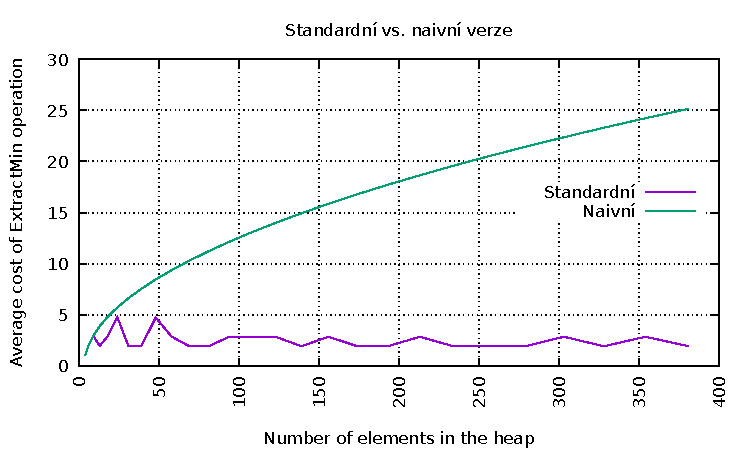
\includegraphics[scale=1.1]{graph_2}		
	\end{figure}

Druhá sada grafů, respektive graf, porovnává naivní implementaci se standardní. Z grafu se zdá, že počet kroků naivní implementace roste přibližně s první odmocninou počtu prvků v haldě.

Tuto hypotézu podporuje i teorie. Pro naivní implementaci totiž, jak mimo jiné říká článek\footnote{Replacing Mark Bits with Randomness in Fibonacci Heaps, Jerry Li, John Peebles 2014} odkazovaný v generátoru, existuje konfigurace haldy a posloupnost operací, která má amortizovanou složitost právě odmocninu z velikosti stormu. 

Konkrétně jde o konfiguraci, kdy les haldy obsahuje stromečky v podobě vždy vrcholu s připojeným jedním synem (bez dalších synů), dvěma syny (bez dalších synů), třema syny, a tak dále. Když pak na této haldě vložíme dvě nová minima a následně provedeme dvakrát delete, tak způsobíme odmocnina mnoho konsolidací (všechny stromy, kterých je právě odmocnina je třbeba při prvním delete sloučit a při druhém zas vrátit do haldového lesa) a vrátíme se do původní konfigurace. Můžeme tedy operaci opakovat a být si jisti, že se neuamortizuje. Multiplikativní konstanta je v tomto případě větší než 1, ale není nikterak extrémně velká. Řádově nízké jednotky. 


\end{document}